\chapter{Proposed Solution}\label{chap:propsol}

\begin{chapquote}{Jim Barksdale}
If we have data, let’s look at data. If all we have are opinions, let’s go with mine.
\end{chapquote}

\section{Introduction}

The purpose of this thesis is to develop a collection of tools for running lightning network 
nodes with daily activity. This requires a data-driven analysis, which involves defining 
and collecting lightning network metrics. In this section, we describe an open-source 
framework for defining and collecting these metrics.

To implement this framework, we conducted an analysis of the state of the art, 
which is described in Section \ref{sec:problem_and_state_of_the_art}. This helped us 
better understand which information is difficult to obtain from a researcher's point 
of view. Our preliminary study revealed that information on how a node performs on a 
daily basis is difficult to obtain due to two primary reasons. First, it requires a direct 
interaction with node operators, who may not be willing to share their data due to 
privacy concerns. Second, data collection of this kind can leak private data, 
and node operators do not want to be exposed to this risk.

To work around these problems, our proposal defines what data will be collected 
and how it will be analyzed in a public manner through a lnmetrics Request for Comments (RFC), 
called \emph{lnmetrics RFC}. Once the data is defined, it is collected using a public 
server with a public API, with the possibility to self-host the server on hardware 
with at least a Raspberry PI 2 capability.

To incentivize node operators to provide and share their information with one
of the public servers available, we developed a tool that collects information on 
the lightning node with the possibility to run in offline mode. Node operators can 
choose whether or not to share their data with one or more of the servers. The ability 
to run the tool in offline mode is a good incentive for node operators to participate 
in the research since they are seeking a tool to analyze the node performance to 
increase their node profit.

Figure \ref{fig:lnmetrics_process} illustrates the general process of how 
our framework works. The process involves five steps:

\begin{figure}
    \begin{center}
      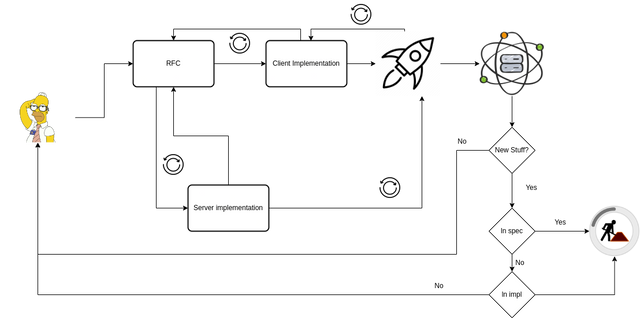
\includegraphics[scale=0.7]{imgs/lnmetrics-workflow-drawio.png}
    \end{center}
    \caption{Example of a process that uses lnmetrics.}
    \label{fig:lnmetrics_process}
\end{figure}


\begin{enumerate}
\item {\bf Data Definition}: The first step involves defining the 
    scope of the data collection.
\item {\bf Client Implementation}: The next step is to implement tools that 
    can collect the data. This step may require going back to the previous step 
        and modifying the data model.
\item {\bf Analysis Implementation}: This step can be done in parallel with the 
    client implementation, and as with the client's case, the analysis of the 
        collected data can lead to a revision of the data model.
\item {\bf RFC Proposal}: When the data model and code are stable, the metric can be proposed 
    with an RFC, and discussions can be held with interested parties. This step may 
        require making changes to one or more of the previous steps.
\item {\bf Possible Proposal}: After the RFC is discussed, the data analysis can lead to an official 
    proposal for the lightning network protocol or one of its implementations.
\end{enumerate}

Section \ref{sec:demo} describes the case study that demonstrates the process we have outlined.

\section{LNMetrics Request for Comments (RFC)}

The LNMetrics Request for Comment (RFC) proposes a more general idea of what has 
already been done in the Lightning Network protocol definition. Its aim is to define
the data that is collected and how it is used, without attempting to establish a standard
of metrics for the Lightning Network. Rather, the RFC aims to encourage discussion
among people to achieve better results.

\subsection{Data Definition}
\label{sec:data_definition}

Data definition is the most important part of proposing a solution to a 
problem that requires data analysis. Therefore, it is a core part of the 
lnmetrics RFC process, as shown in Figure \ref{fig:lnmetrics_process}. The 
process to propose a new metric consists of the following parts:

\begin{itemize}
    \item \textbf{Metric Introduction}: An introduction of the area that the metrics target;
    \item \textbf{Input Metric}: The definition of the data that researchers need. This is done through a JSON Schema.
    \item \textbf{Output Metric}: The definition of the data that the research aims to return as a result.
\end{itemize}

Ideally, a metric proposal should be supported by a reference implementation 
to enable people to participate in the research by running the provided tool and
to support the RFC discussion. However, at present, the problem of how to easily 
integrate new metrics into the existing code is an open problem. One possible 
solution is to allow the server described in Section \ref{sec:lnmetrics_server} 
to support a plugin protocol that allows anyone to extend the existing server 
with additional features and to leave the decision on how to implement the client 
to the user, as described in Section \ref{sec:lnmetrics_client}. In conclusion, 
when a new metric is proposed within the RFC, a discussion between interested 
parties is needed to try to improve and verify the proposal. If this is not 
possible, the proposal can be accepted directly by providing a reference 
implementation of the proposed metrics.

\section{Data Collection with LNMetrics Client}
\label{sec:lnmetrics_client}

An LNMetrics client is a generic tool that can collect one or more metrics
defined within the RFC. It allows a node operator or anyone running a Lightning
node to collect data and share it with an analytical system described in 
Section \ref{sec:lnmetrics_server}. To support our proposal, we provide a
generic solution implemented in Go language, which is available on GitHub
at \url{https://github.com/LNOpenMetrics/go-lnmetrics.reporter}. With this
solution, we were able to provide a generic implementation and support a 
generic metric concept by implementing the metric as an interface, defined
as shown in Listing \ref{code:lnmetric_client_inter}.

\begin{lstlisting}[language=go, basicstyle=\small,
                  caption={Metric interface provided in our client reference implementation.}, 
                  label={code:lnmetric_client_inter}]
// All the metrics need to respect this interface
type Metric interface {
    // return the unique name that the metrics have
    MetricName() *string
    // called when the metrics are initialised from 
    // the lightning node
    OnInit(lightning client.Client) error
    // called when the node is shutting down
    OnStop(msg *Msg, lightning client.Client) error
    // used to make the actual status of the metrics
    // persistent
    MakePersistent() error
    // called when the metrics are ready to be published
    UploadOnRepo(client *graphql.Client, 
        lightning client.Client) error
    // called when the metrics for the specific node 
    //needs to be initialised on the server
    InitOnRepo(client *graphql.Client, 
        lightning client.Client) error
    // call that the lightning node used when it is 
    // time to update the metrics with new data
    Update(lightning client.Client) error
    // a more specific method to be able to call the 
    // update metrics with a specific message that allows 
    // to pass more information to the update method
    UpdateWithMsg(message *Msg, 
        lightning client.Client) error
    ToMap() (map[string]any, error)
    ToJSON() (string, error)
    // allow to perform data migration from an old 
    // data version to a new one
    Migrate(payload map[string]any) error
}
\end{lstlisting}

The provided LNMetrics client uses the core Lightning plugin API, making it 
easy to integrate with the core Lightning daemon and run the metrics client as
part of the node itself. Additionally, to facilitate plugin development, a Go 
API for core Lightning is provided and can be found on Github at \url{https://github.com/vincenzopalazzo/cln4go}.

When the plugin is started, a setup operation is performed by creating a 
metrics database that persists information across node restarts and supports 
the offline mode feature. The chosen database is leveldb, a NO SQL database 
that allows efficient data storage as key-value pairs while also preserving 
disk space with a built-in compression algorithm. Our client implementation 
heavily relies on the compression feature to preserve disk space and enable 
anyone to run the tool. Figure \ref{fig:lnmetrics_diskspace} shows the amount 
of space consumed by the database on our two test machines.

\begin{figure}[H]
    \begin{center}
    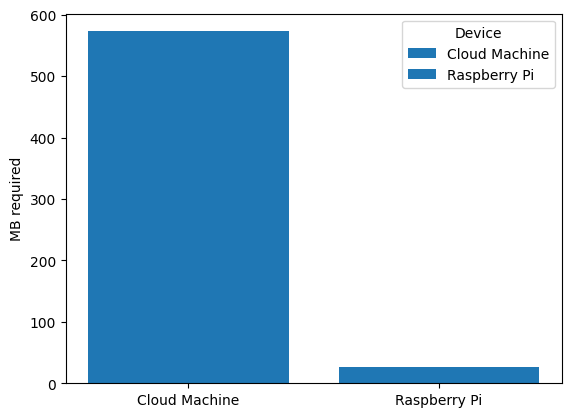
\includegraphics[scale=0.7]{imgs/disk_space_servers.png}
    \end{center}
    \caption{LNMetrics database size by instances.}
    \label{fig:lnmetrics_diskspace}
\end{figure}

In Figure \ref{fig:lnmetrics_diskspace}, a comparison is shown between our two production
machines when we run the lnmetrics framework. We can see that on the {\bf Cloud machine}, the
disk space consumed is around 800 MB to store more than 1 year of node metrics from 3 nodes,
while on a {\bf Raspberry PI 3}, the disk space consumed by the lnmetrics system is less than 100 MB.

There are several reasons for this difference in space between the two machines:

\begin{enumerate}
  \item The cloud machine runs the server with at least 3 nodes in testnet and mainnet for more
        than one year, and these nodes have activities that can include opening and closing channels,
        which require storing some extra bytes for the new channel.
  \item The Raspberry node is newer and has only been running for 3 months, including just one node on
        the Bitcoin network and 3 on the Testnet network.
\end{enumerate}

The point of the figure is to show that the space required to run the system is
orders of magnitude lower than a system that aims to analyze the Bitcoin blockchain.
For example, in \cite{Palazzo_Estrazione_di_Informazioni_2021}, a solution to analyze the Bitcoin blockchain
required 250 GB to store the Bitcoin blockchain and convert it in a compressed JSON format in 2019.
Section \ref{sec:demo} provides more information about the collected data.

\section{Analysis of LNMetrics Data}
\label{sec:lnmetrics_server}

Once the data has been collected using the LNMetrics client described in 
Section \ref{sec:lnmetrics_client}, we propose aggregating it in a server with 
a public API that makes the data publicly accessible to everyone. In this 
section, we discuss the server solution provided.

\subsection{Design Choice}

While aggregating the data collected in a peer-to-peer system in a public 
server may sound a little odd, the LNMetrics framework is designed in a way 
that keeps every concept separate, as shown in Figure \ref{fig:lnmetrics_architecture}. 
The analysis system is independent of the client that collects and reports the data, and
the only information shared across the systems is the data format, which in our
design is done through the LNMetrics RFC.

\begin{figure}
    \begin{center}
    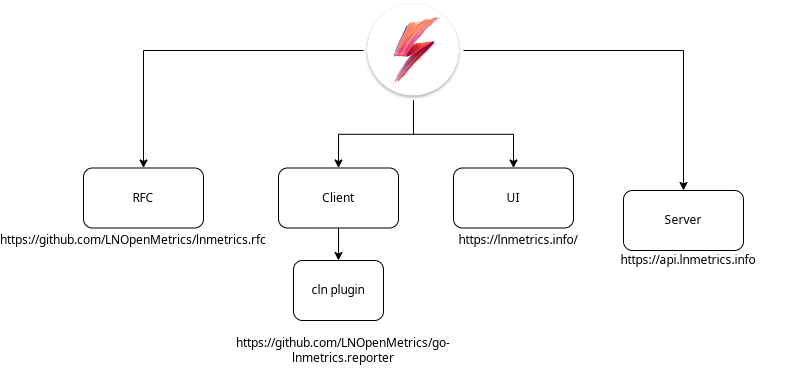
\includegraphics[scale=0.5]{imgs/lnmetrics-architecture.drawio.png}
    \end{center}
   \caption{LNMetrics architecture design diagram.}
    \label{fig:lnmetrics_architecture}
\end{figure}

Our choice to provide the LNMetrics server as a method to analyze the data 
is to give organizations and universities one tool to collect the data in 
a centralized way and simplify the analysis step. However, our client
implementation is able to compute the metric analysis in a local environment 
and allows the owner of the node to inspect the results calculated without 
sharing the data with the centralized server.

\subsection{API Description}

The server API uses the GraphQL protocol, which allows for a flexible way 
to fetch a subset of the data from the server. In particular, the GraphQL 
protocol uses the concept of a query, which makes it possible to specify 
only the data that the caller wants to know and avoid receiving all the JSON 
as a response. The motivation behind this choice is to improve the efficiency 
of the server and speed up performance when the caller needs access to a subset
of information and not the full raw content.

However, the downside of this approach is that the learning curve for a user 
is steeper than with a normal REST protocol. For this reason, we have provided
a Python library that implements a wrap of the server API, which is available
on Github at \url{https://github.com/LNOpenMetrics/py-lnmetrics.api}.

In conclusion, we have provided a public API available at \url{https://api.lnmetrics.info} 
with a website available at \url{https://lnmetrics.info} that provides access to the 
LNMetrics RFC and some analysis of the case study described in the 
following sections.

\section{Local Reputation Metric}
\label{sec:demo}

This section describes our case study that uses the LNMetrics framework 
to define a local reputation of the node to provide a solution to a
problem we encountered while building our lightning node on the
Bitcoin network.

The local reputation described in this section aims to provide enough 
data to support a lightning network user during the initial phase and
helps define some criteria to discover a "good" lightning node where 
it is possible to initialize a channel. In addition, with this local 
reputation system, it is possible to help node management tools, such as
clboss \cite{clboss} to score the channel and have some additional 
information at runtime.


\subsection{Data Definition}
\label{sec:data_definition_datadef}

The first step we took was to design our data model by analyzing the data we 
obtained from the core lightning node. The first version of our data model is 
available on Github at \cite{lnmetrics_localreputation}. The data is divided 
into two main parts, as follows:

\begin{enumerate}
    \item {\bf Lightning Node performance information}: The performance of the node that it is running
        the metrics, including:
        \begin{itemize}
           \item Operative System information;
           \item The number of channels of the node;
           \item The number of forwards payments that the node has performed in the 
               last 30 minutes;
           \item The current lightning fee that the node has to 
               forward a payment.
        \end{itemize}
    \item {\bf Performance for each channel}:
    \begin{itemize}
        \item If the node is online at the moment of the check;
        \item The current lightning fee of the channel to forward a payment through it;
        \item The number of payments that are forwarded in the last 30 minutes through this specific 
            channel;
        \item The channel direction, where for each lightning channel there will be two items: one of 
            inbound connection, and another one for outbound connection. In this way it is possible to 
            try to estimate the usable direction of the channel.
    \end{itemize}
\end{enumerate}

When the client provides the data to the analysis system, the following metric 
output is calculated:

\begin{itemize}
    \item Lightning node up time scoring divided by period is calculated;
    \item Lightning channel forwards payment scoring divided in \emph{success}, \emph{failure}, and \emph{local failure}
        is calculated, where the local failure is how many forwards are failing because of some lightning node problem,
        e.g., the node that is running the metrics has no channel with enough outbound capacity. 
    \item For each channel the previous information is calculated for this particular channel.
\end{itemize}


A more detailed description of the metric output is provided on Github as RFC with 
the  schema of the data just described. We avoid reporting the full code example 
due to the size of the  schema.

\subsection{Reference Implementation}

The client implementation of the local reputation described in Section \ref{sec:data_definition_datadef} 
is provided within our Go Lang reference implementation, already  discussed in Section \ref{sec:lnmetrics_client}. 
This section includes a practical description of how to use it. Therefore, the client implementation is 
a plugin for core lightning that can run as part of the daemon itself. To run the plugin, the core lightning 
needs to know the path of the plugin binary, and an example of the command is shown in
Listing \ref{code:cln_with_lnmetrics}.

\begin{lstlisting}[language=bash, basicstyle=\small,
                  caption={Command to run the core lightning daemon with the lnmetrics plugin enabled.}, 
                  label={code:cln_with_lnmetrics}]
>> lightningd --plugin=/<path to the plugin binary>/go-lnmetrics
\end{lstlisting}

Once the core lightning environment is set up, a directory called \emph{metrics} 
is created within the core lightning directory. This directory is home to the 
lnmetrics plugin, which stores all relevant information. Additionally, a metrics.log 
file is created to facilitate debugging of the plugin without the need to 
interact with the core lightning log daemon.

Upon initialization, the plugin for the local reputation previously described 
initializes the required information. Every 30 minutes thereafter, the plugin
updates metrics by querying the core lightning node for the latest information.

If the plugin is run with the command of Listing \ref{code:cln_with_lnmetrics}, it will run
in offline mode, meaning that metrics will only be stored locally on the node
machine and not shared with the server. To share the data with the server, the 
API URL must be specified, as demonstrated in Listing \ref{code:cln_with_lnmetrics_url}.

\begin{lstlisting}[language=bash, basicstyle=\small,
                  caption={Command to run core lightning with the lnmetrics plugin an publish the data.}, 
                  label={code:cln_with_lnmetrics_url}]
>> lightningd --plugin=/<path to the plugin binary>/go-lnmetrics \ 
--lnmetrics-urls=https://api.lnmetrics.info/query
\end{lstlisting}

More endpoints can be specified by appending them to the "lnmetrics-urls" command line option, separated by a comma.

In conclusion, the plugin can be queried by interacting with the core lightning 
command line interface and calling the methods provided by the plugin:

\begin{itemize}
    \item {\bf raw-local-reputation}: This endpoint allows one to query the most recent input data 
        collected by the plugin in the past 30 minutes. The data format for this endpoint 
        is described in \cite{lnmetrics_localreputation}.
    \item {\bf local-reputation}: This endpoint allows one to query the most recent local 
        reputation score calculated using the data provided by the raw-local-reputation 
        endpoint. The data format for this endpoint is also described in \cite{lnmetrics_localreputation}.
\end{itemize}

\subsection{Data Analysis}

When the client is running with an endpoint, as shown in Listing \ref{code:cln_with_lnmetrics_url}, the metrics are 
collected and reported to the specified server. The server instance exposes an endpoint that accepts a \emph{Mutation} 
query, as shown in Listing \ref{code:lnmetrics_mutation}.

\begin{lstlisting}[language=graphql, basicstyle=\small,
                  caption={Mutation query call by the client to initialise the metric on the server.}, 
                  label={code:lnmetrics_mutation}]
mutation {
    initMetricOne(node_id: "...", payload: "{....}", signature: "...") {
        node_id
        ...
    }
}
\end{lstlisting}

The mutation query accepts the following input parameters:

\begin{itemize}
    \item {\bf node\_id}: The node public key used as the node identifier on the lightning network.
    \item {\bf payload}: The JSON payload of the metric that the node is publishing.
    \item {\bf signature}: The signature of the JSON payload sent as input to verify that the
        payload is sent by the node with the provided public key.
\end{itemize}

The algorithm used to sign the payload is a custom one provided by the major
lightning implementation, and we provide our own Go implementation, which is available
at \url{https://github.com/LNOpenMetrics/lnmetrics.utils}.

Once the server accepts and verifies the metrics, it will analyze the provided data and calculate the
metrics output described in section \ref{sec:data_definition_datadef}. The metrics will then be available
through the server endpoint. Additionally, our Python client provides an easy API to access any server instances.
Listing \ref{code:lnmetrics_python_api} provides a runnable example.

\begin{lstlisting}[language=python, basicstyle=\small,
                  caption={Python script to show a runnable example of our Python wrapper API usage.}, 
                  label={code:lnmetrics_python_api}]
from lnmetrics_api import LNMetricsClient

client = LNMetricsClient(service_url="https://api.lnmetrics.info/query")
nodes = client.get_nodes(network="bitcoin")
print(f"The nodes on the server are {nodes}")
metric = client.get_local_score_output(network="bitcoin", 
               node_id="03e2408a49f07...")
print(f"The local score of the node is {metric}")
\end{lstlisting}

In addition, we have used the Python API to create a Jupyter Notebook, which 
is available at \url{https://github.com/LNOpenMetrics/local-reputation-analysis}.
In the notebook, we perform an initial analysis of the collected data and discuss 
the results in the remaining sections.

\subsubsection{Nodes Up time}
\label{sec:node_uptime}
This section presents the results of the analysis of metrics provided by the
nodes available on the cloud server.

\begin{figure}
    \begin{center}
      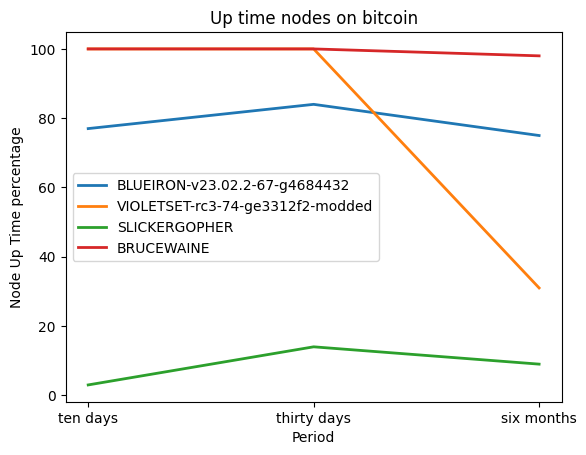
\includegraphics[scale=0.7]{imgs/bitcoin_uptime.png}
    \end{center}
    \caption{Lightning Node up-time scoring on the Bitcoin Network calculated by the cloud machine.}
    \label{fig:lnmetrics_uptime_bitcoin}
\end{figure}

\begin{figure}
    \begin{center}
      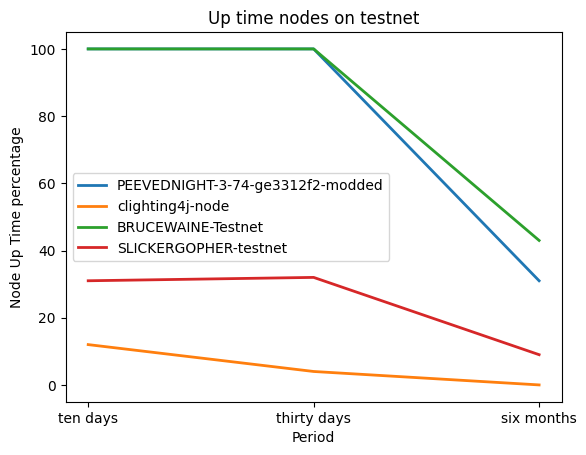
\includegraphics[scale=0.7]{imgs/testnet_uptime.png}
    \end{center}
    \caption{Lightning Node up-time scoring on the Testnet Network calculated by the cloud machine.}
    \label{fig:lnmetrics_uptime_testnet}
\end{figure}

Figure \ref{fig:lnmetrics_uptime_bitcoin} shows the uptime scores
of the nodes that share data on the server every 30 minutes.
The node with 100\% uptime is always online. From this analysis,
we can observe certain patterns where some nodes are not always
online, such as the node with the alias \emph{SLICKERGOPHER}.
This node is not a routing node, but it is run by a casual user.
However, in most cases, the casual user uses the Tor Network \cite{tor}
to expose the {\LN} node to the public without using a public IP
that can leak private data on the user position. Therefore, a node
that uses only tor can be flaky in availability due to some network
problems caused by some Tor relay nodes being overloaded.

A possible future work could be an analysis of the up-time of a node
in two different zones of the world that use only the Tor network to
be a routing node. In this case, we may see that the Tor network may
impact the uptime performance if the node is located in an overloaded
area, and if this impacts the network view of the node, such as the
belief that a node is reachable because it is online, but it is
not because the other nodes cannot connect to it through the Tor network.

In conclusion, Figure \ref{fig:lnmetrics_uptime_testnet} shows the uptime of
the nodes in the Testnet network, where we can also observe this
difference between nodes that are always online and casual users.

\subsubsection{Forwards Rating}
\label{sec:forwards_rating}

In Section \ref{sec:node_uptime}, we analyzed the uptime of the nodes 
and noted that there are at least two kinds of nodes:

\begin{itemize}
    \item {\bf Routing Node}: Nodes that are always online;
    \item {\bf Casual User Node}: Nodes that are not always online.
\end{itemize}

Therefore, just analyzing the uptime of a node is not enough to estimate if a node is a 
good node for the public network because a routing node that is always online needs to 
have some activity, and this activity should not be dangerous for the network.
For this reason, in this section, we use the forwards rating to measure the activity of 
a node by analyzing how many payments are forwarded by the routing node under analysis. 
For our analysis, we consider two nodes, one in the Bitcoin Network and the other 
one in the Testnet network:

\begin{itemize}
    % FIXME: there is a better way to go to the next line, but I am not able to find this better way!
    \item {\bf BLUEIRON}: The lightning node with the public key 024b9a1fa8e006f1e3937f6-\\5f66c408e6da8e1ca728ea43222a7381df1cc449605 for the Bitcoin Network;
    \item {\bf BRUCEWAINE-Testnet}: The lightning node with public key 030b686a163aa2bba0-\\3cebb8bab7778fac251536498141df0a436d688352d426f6 for the Testnet Network.
\end{itemize}

Figure \ref{fig:bitcoin_vs_testnet_forwards} shows an analysis of the forwarded 
payments by the node under analysis for each network, and Figure \ref{fig:bitcoin_vs_testnet_channels_size} 
shows an analysis of the size of the node during the period that includes the number
of channels that the node has.

Therefore, from this comparison, we can see that the activity on the Bitcoin network is an order of magnitude
bigger than the activity on the Testnet network, even if the size of the node is close to the same. This 
shows that the activity on the Bitcoin network and the activity on the Testnet network are very different,
and this may impact the proposal evaluation that is dependent on the network, such as the local scoring 
proposed by the solution to solve the Jamming Attack discussed in Section \ref{sec:jamming}.

\begin{figure}[H]
    \begin{center}
        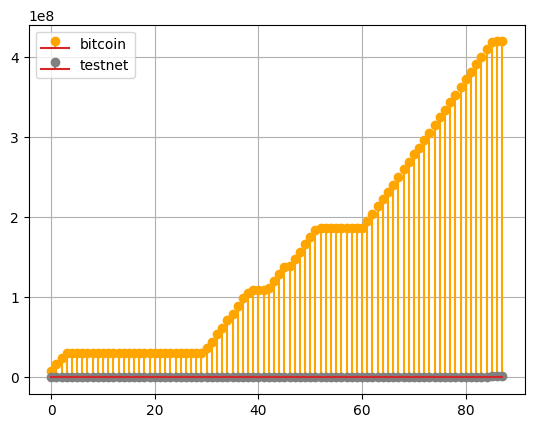
\includegraphics[scale=0.7]{imgs/bitcoin_vs_testnet_forwards.png}
    \end{center}
    \caption{Comparison between networks of the Lightning Node forwards scoring.}
    \label{fig:bitcoin_vs_testnet_forwards}
\end{figure}

\begin{figure}[H]
    \begin{center}
      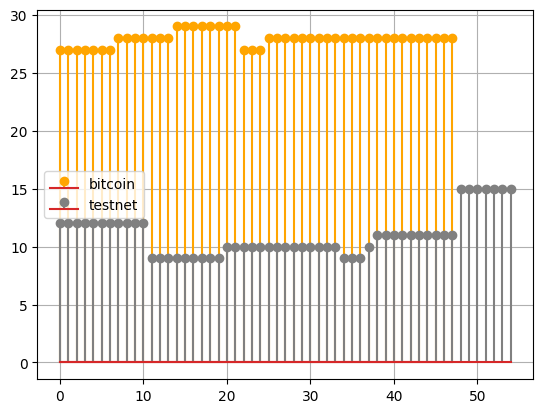
\includegraphics[scale=0.7]{imgs/bitcoin_vs_testnet_channels_size.png}
    \end{center}
    \caption{Comparison between networks of the Lightning Node size.}
    \label{fig:bitcoin_vs_testnet_channels_size}
\end{figure}

However, as shown in Figure \ref{fig:bitcoin_forwards_rating}, we can see that the success
forward scoring on the Bitcoin network is also close to 5\% of the total forwards performed 
in the last 6 months. One of the main reasons for this result could be the probing techniques 
used by some nodes to estimate the exact capacity of the channel before performing the path-finding
algorithm. In these probing techniques, the node that wants to make payments sends fake payments
that are already destined to fail, with an increasing amount, just to determine if the channel 
is able to forward it. The lightning node that receives this forward payment is not able to 
detect that it is a fake payment due to the onion routing discussed in Section \ref{sec:onion_routing}.

Therefore, relying solely on a node's global forward scoring is not enough, as the failure
scoring will always be a significant aspect of this analysis due to the probing techniques
used. However, this information can still be useful in filtering out nodes that only
forward failed payments and are not subject to local failures. It is assumed that a node
that sends many payments but none of them result in successful completion is not useful.

\begin{figure}[H]
    \begin{center}
      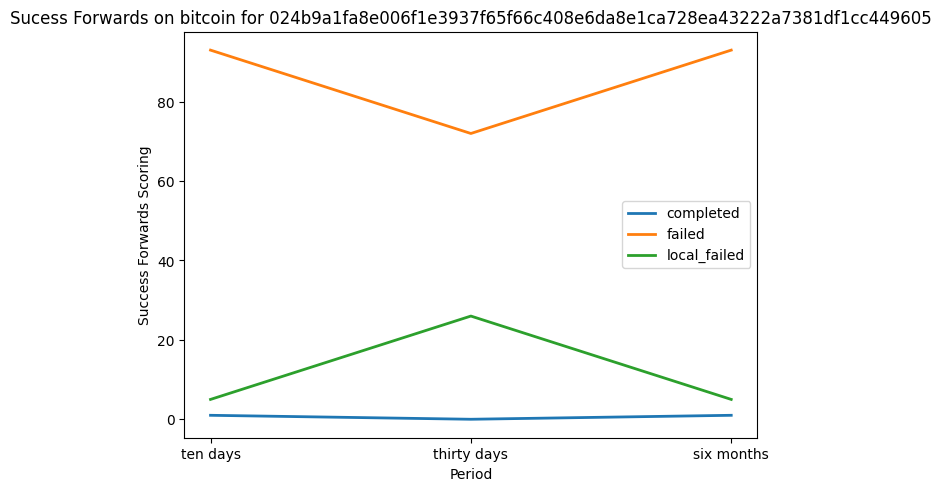
\includegraphics[scale=0.7]{imgs/bitcoin_forwards_rating.png}
    \end{center}
    \caption{Forwards Scoring for the Lightning network node on the Bitcoin Network.}
    \label{fig:bitcoin_forwards_rating}
\end{figure}

% FIXME: we could add a small analysis of the forwards scoring for each channels has
